\documentclass[12pt, a4paper, headings=normal]{article}
\usepackage[polish]{babel}
\usepackage[utf8x]{inputenc}
\usepackage[T1]{fontenc}
\usepackage{polski}
\usepackage{graphicx}
\usepackage{amsmath}
\usepackage{csvsimple}
\usepackage{float}
\usepackage{geometry}
\usepackage[font=small]{caption}
\usepackage{subcaption}
\usepackage{fancyhdr}
\usepackage{hyperref}
\usepackage{gensymb}
\usepackage{lscape}
\usepackage{tikz}

\hypersetup{
	colorlinks=true,
	linkcolor=black,
	filecolor=magenta,      
	urlcolor=black,
}


\newgeometry{tmargin=2cm, bmargin=2cm, lmargin=2.5cm, rmargin=2.5cm}

\setlength{\parindent}{10pt}
\graphicspath{{../img}}
\addto\captionspolish{\renewcommand{\figurename}{Rys.}}

\pagestyle{fancy}
\rhead[]{Michał Łukaszewicz (297696)}
\lhead[]{PSM: Projekt 2}

\begin{document}

\begin{titlepage}

   \begin{figure}
        \begin{subfigure}{.5\linewidth}    
            \centering
            
\includegraphics[width=.6\linewidth]{pw_logo.png}
        \end{subfigure}
        \begin{subfigure}{.5\linewidth}    
            \centering
            
\includegraphics[width=.6\linewidth]{simr_logo.jpg}
        \end{subfigure}
    \end{figure}

	\begin{center}
		
	\vspace*{0.2\textheight}

	\begin{Large}
	\textbf{Projektowanie Systemów Mechatronicznych}
	\end{Large}

	\vspace{0.5cm}
	
	\begin{large}
		PROJEKT 2\\
		Projekt układu sterowania tempomatu aktywnego
	\end{large}
	
	\vspace{1.5cm}

	\textbf{Michał Łukaszewicz (297696)}

	\vfill

	Wydział Samochodów i Maszyn Roboczych\\
	Politechnika Warszawska\\
	2021
	
		
	\end{center}
\end{titlepage}
\newpage

\tableofcontents

\newpage
\section{Cel i założenia}

Celem projektu jest stworzenie modelu pojazdu Mitsubishi Lancer 1.5 i zaprojektowanie 
dla niego układu regulacji spełniającego rolę tempomatu aktywnego.

\subsection{Dane}

Parametry pojazdu:
\begin{itemize}
	\item Masa własna - $m = 955$ kg
	\item Powierzchnia czołowa - $A = 2.18 m^2$
	\item Współczynnik oporów powietrza - $c_x = 0.3$
	\item Współczynnik oporów toczenia - $f_0 = 0.01$
	\item Sprawność układów mechanicznych - $\eta = 0.9$
	\item Promień dynamiczny - $r_d = 0.36$ m
	\item Maksymalna siła hamowania - $F_{brk-max} = 7500$ N
\end{itemize}

% charakterystyka prędkościowa

\begin{figure}[H]
	\centering
	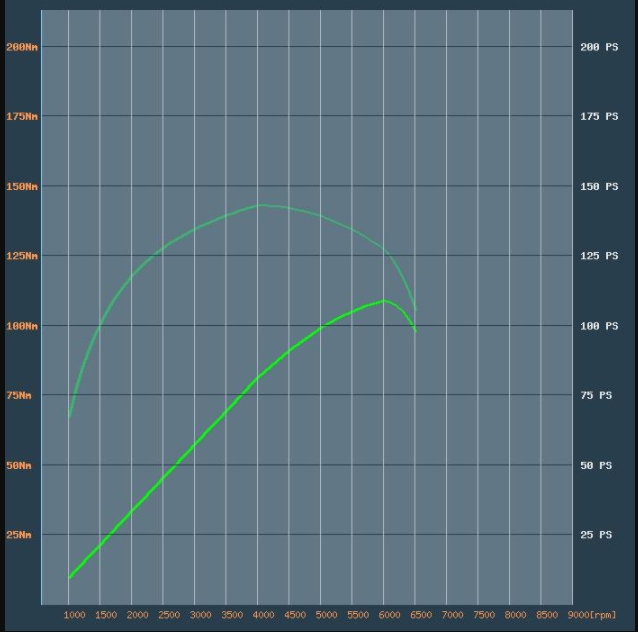
\includegraphics[width=.8\textwidth]{trq_auto.jpg}
	\caption{Charakterystyka szybkościowa silnika \cite{autocatalog}}
	\label{fig:trq_auto}
\end{figure}

\section{Opis matematyczny badanego obiektu}

Ruch pojazdu można opisać równaniem z \cite{arczy}:

\begin{equation}
	\label{eq:dyn1}
\begin{array}{c}
	F_n - \sum F_{op} = 0 \\
	F_n = F_t + F_p + F_w + F_i + F_u + F_s\\
\end{array}
\end{equation}

Gdzie: $F_t$ - siła oporów toczenia, $F_p$ - siła oporów powietrza, $F_w$ siła oporów
wzniesienia, $F_b$ - siła oporów bezwładności, $F_u$ - siła oporów uciągu, 
$F_s$ - siła oporów skrętu.

Pojazdy w symulacji będą poruszały się w linii prostej po płaskiej nawierzchni ($\alpha = 0$),
bez dodatkowych przyłączonych przyczep, dzięki czemu równanie \eqref{eq:dyn1} upraszcza się
do postaci:

\begin{equation}
	\label{eq:dyn2}
\begin{array}{c}
	F_n = F_t + F_p + F_b \\
\end{array}
\end{equation}

Gdzie korzystając z bezwładności masy skupionej możemy przekształcić:

\begin{equation}
	\label{eq:dyn3}
\begin{array}{c}
	F_b =  m \ddot{x} \\
	m \ddot{x} = F_n - F_t - F_p\\
\end{array}
\end{equation}

Równanie \eqref{eq:dyn3} możemy rozwinąć o składową hamowania $F_{brk}$ uzyskując
końcową postać równania ruchu pojazdu \eqref{eq:dyn4}.

\begin{equation}
	\label{eq:dyn4}
\begin{array}{c}
	m \ddot{x} = F_n - F_t - F_p - F_{brk}\\[10pt]
	\ddot{x} = \dfrac{F_n - F_t - F_p - F_{brk}}{m}\\
\end{array}
\end{equation}

Poszczególne składowe obliczamy z następujących zależności:

\begin{equation}
\begin{array}{l}
	F_t = m g \cdot f_0 \\
	F_p = c_x \cdot A \cdot \rho_{air} \cdot \dfrac{v^2}{2}
	\label{eq:drags}
\end{array}
\end{equation}

Siła napędowa oraz siła hamowania wynikają z parametrów pojazdu. 

\section{Model w środowisku MATLAB/Simulink}

Uruchomienie symulacji realizowane jest w skrypcie \textit{simul.mlx}

\subsection{Założenia przyjęte w modelu}

\subsubsection{Charakterystyka ruchu}

Pojazdy poruszają się we wspólnym jednowymiarowym układzie odniesienia wzdłuż
ustalonej osi \textit{s}, pojazd wiodący oznaczono jako \textit{car2}, pojazd
podążający jako \textit{car1}. Odległość pomiędzy pojazdami $\Delta s$ jest równa
różnicy odległości pojazdów od początku układu współrzędnych - $\Delta s = s_2 - s_1$

\begin{figure}[H]
	\centering
	\begin{tikzpicture}
		\draw[black, thick, -latex] (0,0) -- (10,0);
		\node[below] at (10, 0) {\textit{s}};
		% car1
		\draw[] (1, 0.1) circle (0.1);
		\draw[] (1 + 0.5, 0.1) circle (0.1);
		\draw[] (1 - 0.25, 2*0.1) rectangle (1-0.25+1, 0.8)
		node[pos=.5] {car1};
		\draw[-latex] (1-0.25, 1.1) -- (2-0.25, 1.1)
		node[pos=.5, above] {$v_1$};
		% car2	
		\draw[] (7, 0.1) circle (0.1);
		\draw[] (7 + 0.5, 0.1) circle (0.1);
		\draw[] (7 - 0.25, 2*0.1) rectangle (7-0.25+1, 0.8)
		node[pos=.5] {car2};
		\draw[-latex] (7-0.25, 1.1) -- (8-0.25, 1.1)
		node[pos=.5, above] {$v_2$};
		%distance
		\draw[black, thick, <->] (2-0.25, 0.5) -- (7-0.25, 0.5);
		\node[above] at (8.5/2, 0.5) {$\Delta s$};
	\end{tikzpicture}
	\caption{Schemat symulowanego zdarzenia}
\end{figure}

\subsubsection{Parametry pojazdu}

Charakterystyka szybkościowa została przybliżona wielomianem drugiego stopnia
dla ułatwienia implementacji w modelu, do przybliżenia wykorzystano funkcję \textit{polyfit} i w wyniku
otrzymano funkcję wielomianową w postaci:
\begin{equation}
	M_{max} = -6.6774 \cdot 10^{-6} \cdot n^2 + 0.056 n + 27.2132
	\label{eq:trq_poly}
\end{equation}

\begin{figure}[H]
	\centering
	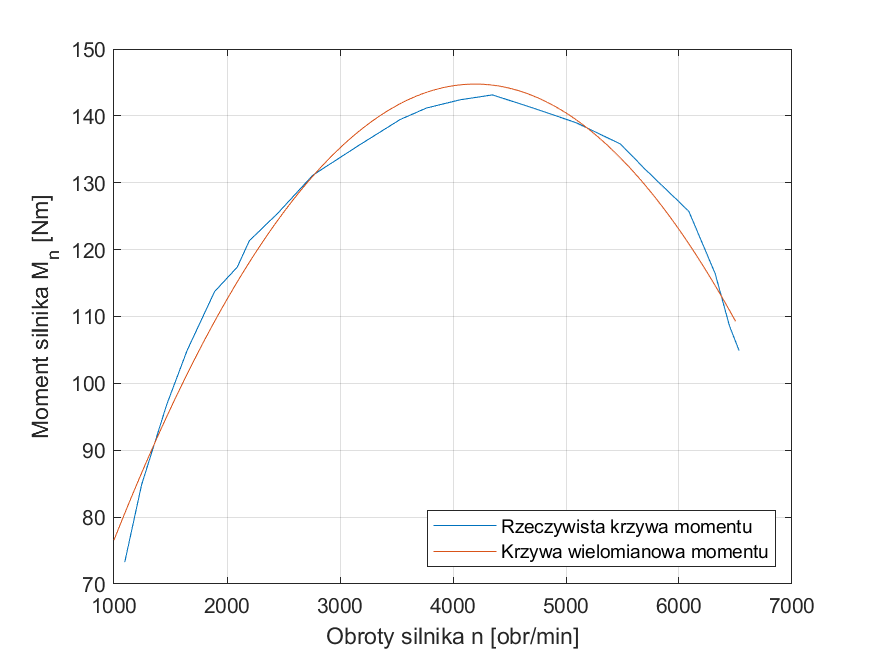
\includegraphics[width=.7\textwidth]{trq_curve.png}
	\caption{Charakterystyka szybkościowa i jej przybliżenie krzywą wielomianową}
	\label{fig:trq_curve}
\end{figure}


\subsection{Implementacja modelu matematycznego}

\begin{figure}[H]
	\centering
	\includegraphics[width=.9\textwidth]{"eq_model.png"}
	\caption{Subsystem \textit{Motion Equations} - implementacja równań ruchu}
	\label{fig:mtneqs}
\end{figure}

Równanie ruchu pojazdu zaimplementowano wewnątrz subsystemu \textit{Motion Equations},
przyjmującego dwa parametry wyjściowe: \textit{Torque} - Moment na kołach oraz
\textit{Brake \%} - zadany procent maksymalnej siły hamowania. Wyjścia z subsystemu
przedstawiają kolejno: \textit{a} - $\ddot{s}$ - przyśpieszenie pojazdu, \textit{v} -
$\dot{s}$ - prędkość pojazdu oraz \textit{s} - drogę przebytą przez pojazd (w globalnym
układzie odniesienia s)

Dla uzyskania siły napędowej $F_n$ moment na wejściu dzielony jest przez promień dynamiczny
koła $r_d$. Wartości siły oporów toczenia oraz oporów powietrza wynikają z \eqref{eq:drags}. Siła
hamowania jest uzyskiwana poprzez przemnożenie wejścia \textit{Brake \%} poprzez wartość
maksymalnej siły hamowania.

\subsection{Symulacja podzespołów pojazdu}

Dla uzyskania bliskiej rzeczywistości symulacji pojazdu należy zaimplementować w 
modelu dodatkowe elementy odpowiedzialne za przełożenia istniejące w układzie napędowym
oraz zdolność silnika do wygenerowania momentu w różnych zakresach prędkości obrotowych.

\begin{figure}[H]
	\centering
	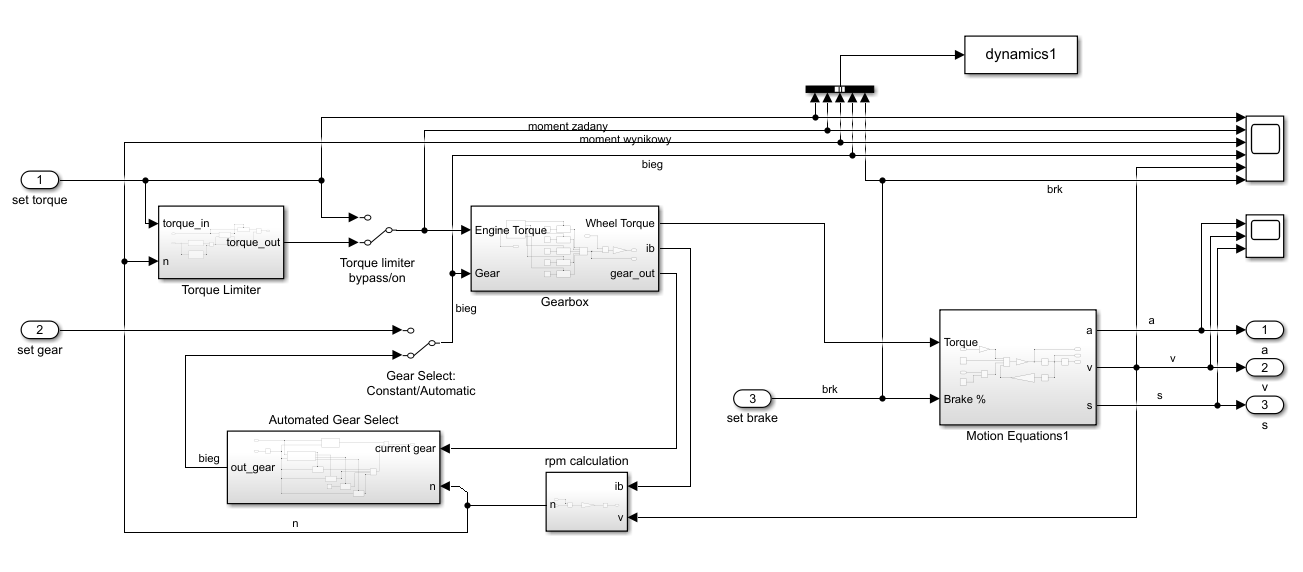
\includegraphics[width=\textwidth]{cardynamics.png}
	\caption{\textit{Car Dynamics} - schemat subsystemu}
	\label{fig:cardynamics}
\end{figure}

Na Rys. \ref{fig:cardynamics} przedstawiono układ symulujący zachowanie pojazdu,
wykorzystuje on subsystem \textit{Motion Equations} z Rys. \ref{fig:mtneqs} współpracujący z
dodatkowymi subsystemami: \textit{Gearbox} - symulacja skrzyni biegów, \textit{Torque Limiter} -
symulacja podaży momentu silnika, \textit{Automated Gear Select} - 'automatyzacja' 
wyboru przełożeń skrzyni biegów, \textit{rpn calculation} - moduł obliczający prędkość
obrotową silnika.

\bigskip

Model został stworzony zgodnie z koncepcją bottom-up czyli projektowania podzespołów
składowych w pierwszej kolejności a następnie integracji ich w nadrzędne systemy. 
Dzięki temu każdy włączany do modelu system może być przetestowany w pracy samodzielnie
i po potwierdzeniu jego sprawności wyłączany z poszukiwania błędów w systemie nadrzędnym.

\subsubsection{Torque Limiter - ogranicznik momentu}

\begin{figure}[H]
	\centering
	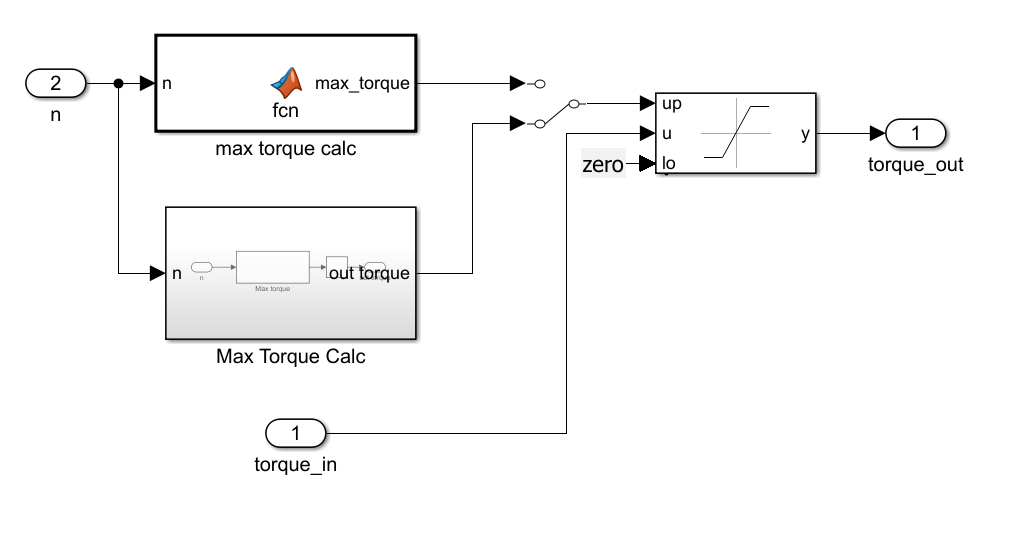
\includegraphics[width=.8\textwidth]{torquelimiter.png}
	\caption{\textit{Torque Limiter} - schemat subsystemu}
	\label{fig:torquelimiter}
\end{figure}

Ogranicznik momentu uzależnia moment możliwy do przekazania na koła od prędkości
obrotowej silnika symulując przebieg charakterystyki prędkościowej na podstawie
krzywej wielomianowej opisanej na Rys. \ref{fig:trq_curve} i \eqref{eq:trq_poly}.

Dla momentu zadanego $M_{zad}$ oraz maksymalnego dostępnego momentu $M_{max}$ obliczonego
z \eqref{eq:trq_poly} układ realizuje funkcję:

\begin{equation}
	M_{wynikowy} = \left\{ \begin{array}{l c r}
		M_{zad} & dla & M_{zad} < M_{max} \\
		M_{max} & dla & M_{zad} > M_{max} \\
	\end{array}\right.
\end{equation}

\subsubsection{Gearbox - skrzynia biegów}

\begin{figure}[H]
	\centering
	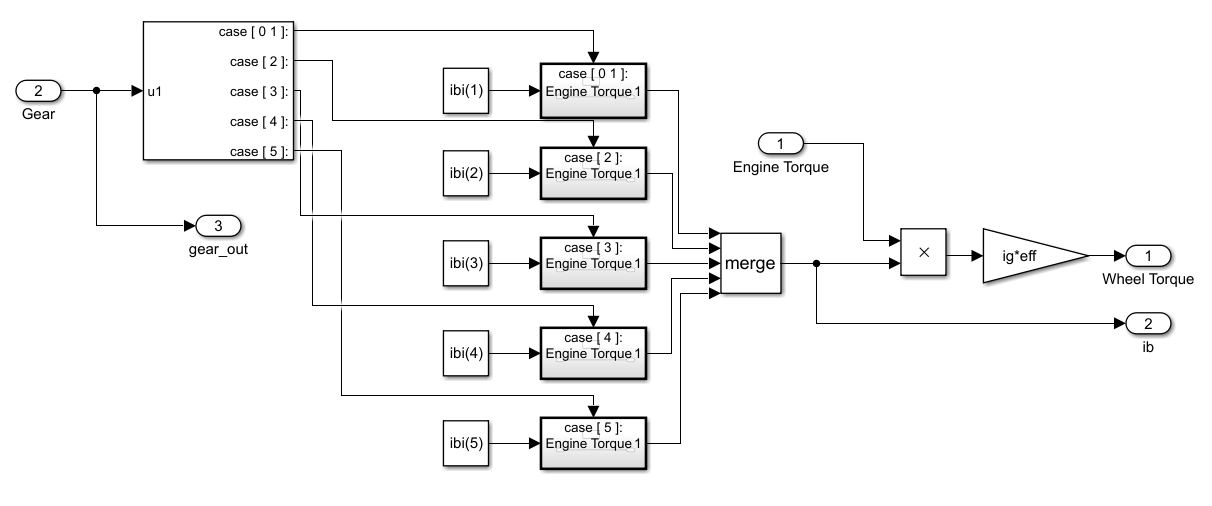
\includegraphics[width=\textwidth]{gearbox.png}
	\caption{\textit{Gearbox} - schemat subsystemu}
	\label{fig:gearbox}
\end{figure}

Celem zastosowania skrzyni biegów jest zapewnienie aby przełożenie momentu na koła
w różnych zakresach prędkości poruszania się pojazdu miało wartość umożliwiającą
utrzymanie prędkości obrotowej w zakresie największych wartości momentu napędowego.

W zastosowanym układzie struktura warunkowa \textit{case} wybiera przełożenie na podstawie
parametru wejściowego \textit{2: Gear}, następnie dokonuje obliczenia momentu na kołach
wykorzystując parametr wejściowy momentu silnika \textit{1: Engine Torque}, przełożenie
przekładni głównej $i_g$ oraz parametr sprawności układów mechanicznych $\eta$ (oznaczony w modelu
jako \textit{eff}). 

\begin{equation}
	\begin{array}{l c r}
		M_{nk} = M_n \cdot i_b  i_g \eta & dla & i_b =  \left\{ \begin{array}{l r}
			3.31 & \text{Bieg 1}\\
			1.91 & \text{Bieg 2}\\
			1.31 & \text{Bieg 3}\\
			0.97 & \text{Bieg 4}\\
			0.81 & \text{Bieg 5}\\
		\end{array}\right.
	\end{array}
\end{equation}

Subsystem zwraca wybrany bieg, wartość przełożenia i obliczony moment na kołach.

\subsubsection{Automated Gear Select - automatyczny selektor biegów}

\begin{figure}[H]
	\centering
	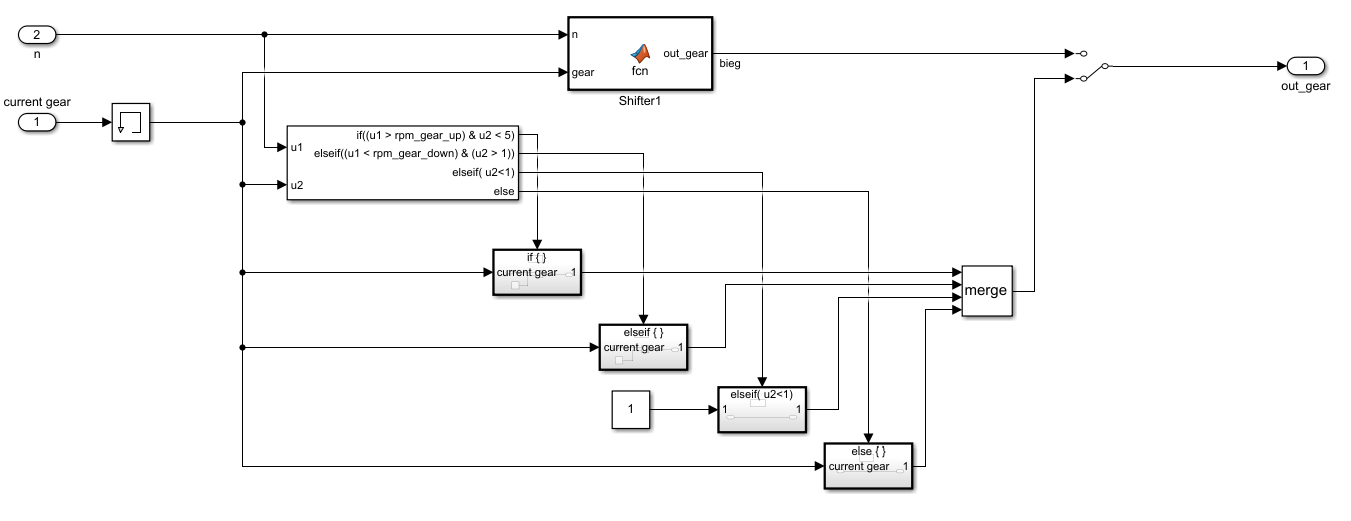
\includegraphics[width=\textwidth]{gearselector.png}
	\caption{\textit{Automated Gear Select} - schemat subsystemu}
	\label{fig:autogear}
\end{figure}

Aby nie nie było konieczne manualne generowanie sygnału sterującego skrzynią biegów
zastosowano system dokonujący automatycznej selekcji biegu na podstawie prędkości
obrotowej wału silnika $n$.

Subsystem przyjmuje jako parametry wejściowe: \textit{1: current gear} - informację
o obecnie ustawionym biegu oraz \textit{2: n} - prędkość obrotową wału silnika. Na
podstawie wartości wejściowych oraz zmiennych skryptu konfiguracyjnego: \textit{rpm\_gear\_up} oraz
\textit{rpm\_gear\_down} dokonuje selekcji biegu zgodnie z funkcją:

\begin{equation}
	\textit{set\_gear} = \left\{ \begin{array}{l c l}
		\textit{current gear} + 1 & dla & n > \textit{rpm\_gear\_up} \text{ \& } \textit{current gear} < 5 \\
		\textit{current gear} - 1 & dla & n < \textit{rpm\_gear\_down} \text{ \& } \textit{current gear} > 1 \\
		1 & dla & \textit{current gear} < 1 \\
		\textit{current gear} & dla & \textit{rpm\_gear\_down} < n < \textit{rpm\_gear\_up}
	\end{array}
	\right.	
\end{equation}

Dodatkowo dla zabezpieczenia przed wystąpieniem pętli algebraicznej w torze wejścia
\textit{1: current gear} zastosowano blok \textit{Memory} opóźniający wejście danych o jeden
cykl.

\subsubsection{RPM calculator - obliczanie prędkości obrotowej silnika}

\begin{figure}[H]
	\centering
	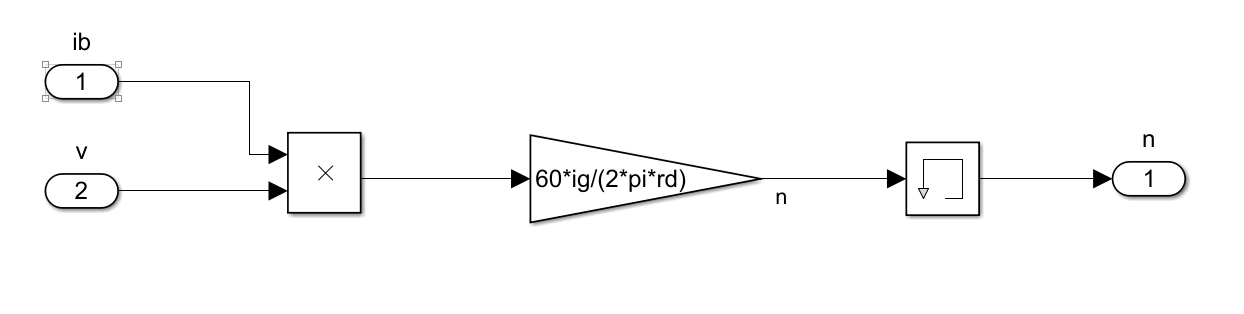
\includegraphics[width=\textwidth]{rpmcalc.png}
	\caption{\textit{rpn calculator} - schemat subsystemu}
	\label{fig:rpmcalc}
\end{figure}

Prędkość obrotowa silnika obliczana jest na podstawie prędkości poruszania się pojazdu oraz
parametrów przełożenia skrzyni biegów, zgodnie z następującą formułą:

\begin{equation}
	n = \dfrac{60 \cdot v \cdot i_b i_g}{2 \pi r_d}
	\label{eq:rpmeq}
\end{equation}

Dla zabezpieczenia przed wystąpieniem pętli algebraicznej wykorzystano blok \textit{Memory}
podobnie jak w subsystemie \textit{Autmoated Gear Select}.

\subsubsection{Dodatkowe opcje konfiguracyjne}

Model pojazdu skonstruowany w ten sposób może powodować trudności w strojeniu układu
regulacji, aby uniknąć tego problemu zastosowano przełączniki obejścia dla subsystemów
\textit{Torque Limiter} oraz \textit{Automated Gear Select}. 

W przypadku układu \textit{Torque Limiter} w trybie obejścia ("bypass") moment zadany
traktowany jest jako moment wynikowy i przekazywany do skrzyni biegów. Uruchomienie
trybu obejścia dla układu \textit{Automated Gear Select} uaktywnia parametr wejściowy
\textit{2: set gear}, za pomocą którego ręcznie należy ustawić pożądany bieg.

\begin{figure}[H]
	\centering
	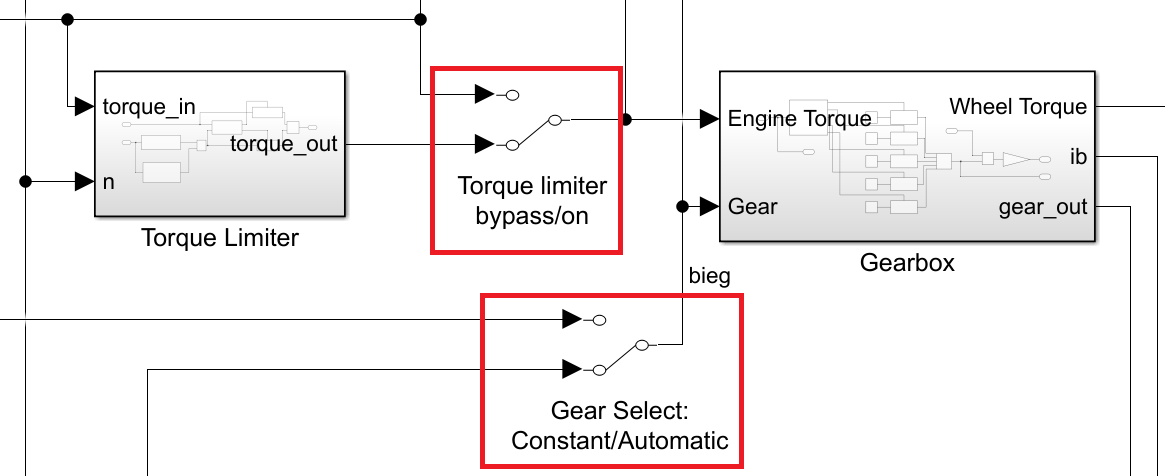
\includegraphics[width=.8\textwidth]{bypass.png}
	\caption{Przełączniki układów obejścia w subsystemie \textit{Car Dynamics}}
	\label{fig:bypass_sw}
\end{figure}

\subsection{Układ sterowania}

Układ tempomatu składa się z dwóch bloków zadaniowych: \textit{Speed} - bloku tempomatu
pasywnego czyli dążącego do utrzymania zadanej prędkości, \textit{Distance} - bloku tempomatu
aktywnego dążącego do utrzymania zadanego dystansu do poprzedzającego pojazdu.

Tempomat może działać w trybie preferencji jednego z bloków, lub w trybie automatycznym
w, którym jeżeli w zasięgu czujników (w tym przypadku teoretycznych) pojawia się pojazd,
to układ będzie starał się utrzymywać do niego zadaną odległość, mając jednocześnie
zadany warunek maksymalnej prędkości o wyższym priorytecie niż warunek dystansu.
 

\newpage
\begin{landscape}
	\begin{figure}
		\centering
		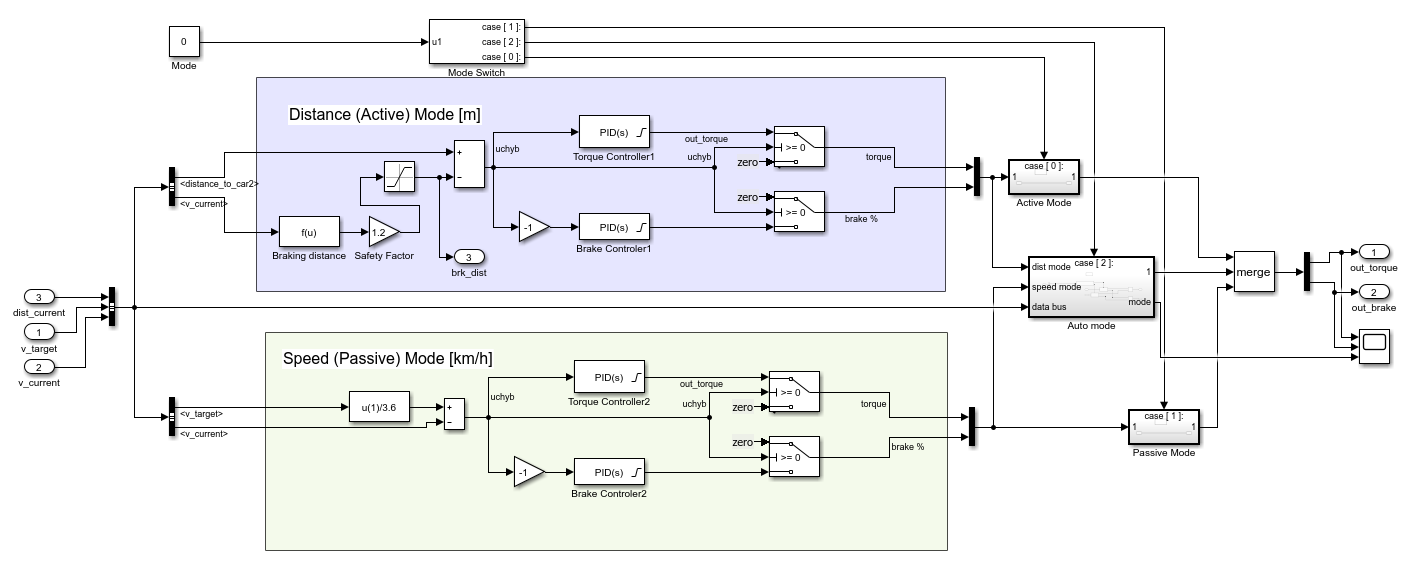
\includegraphics[width=\linewidth]{tempomat.png}
		\caption{Układ tempomatu}
		\label{fig:tempomat}
	\end{figure}	
\end{landscape}


\subsubsection{Tempomat - blok pasywny}

\begin{figure}[H]
	\centering
	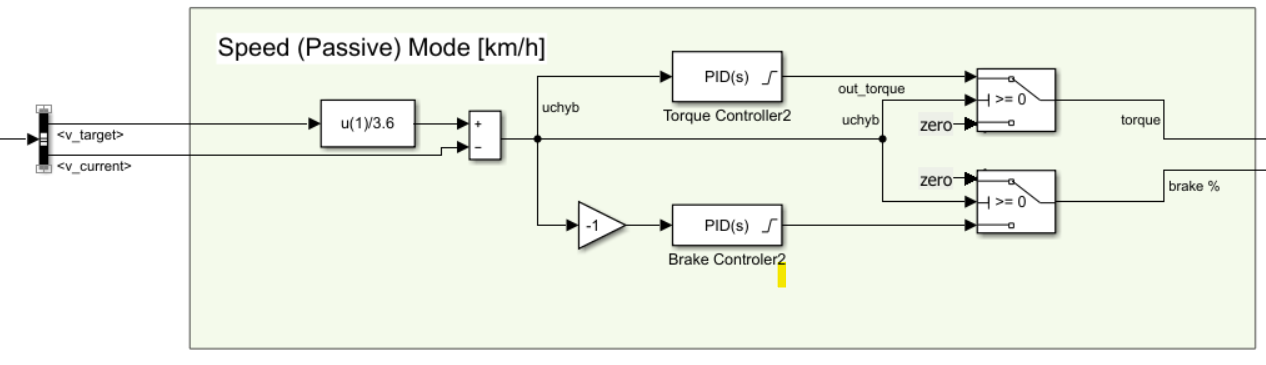
\includegraphics[width=\textwidth]{tempo_pass.png}
	\caption{Blok tempomatu pasywnego}
	\label{fig:tempo_pass}
\end{figure}

Blok pasywny tempomatu ma za zadanie utrzymanie zadanej prędkości. Do układu podawana
jest chwilowa prędkość poruszania się pojazdu oraz zadana wartość prędkości z jaką pojazd
ma się poruszać.

\subsubsection{Tempomat - blok aktywny}

\begin{figure}[H]
	\centering
	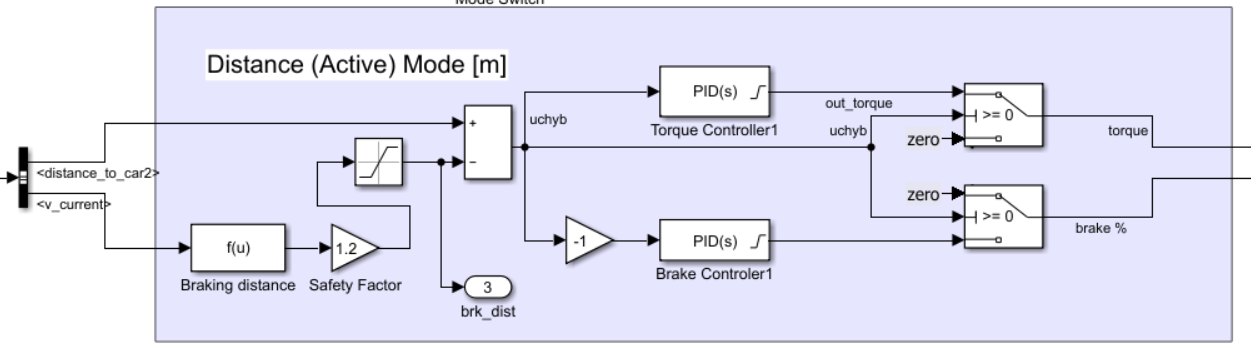
\includegraphics[width=\textwidth]{tempo_act.png}
	\caption{Blok tempomatu aktywnego}
	\label{fig:tempo_act}
\end{figure}

Blok aktywny różni się od pasywnego korzystaniem z informacji o odległości do pojazdu
wiodącego (obliczanej poza systemem tempomatu) zamiast z informacji o prędkości, ponadto
w bloku aktywnym nie zadajemy wartości dystansu, który ma być utrzymywany, wielkość 
tą obliczamy z zależności na drogę hamowania z uwzględnieniem współczynnika bezpieczeństwa:

\begin{equation}
	\label{eq:temp_act_dist}
	\begin{array}{c}
	s_{brk} = v_0 \cdot t_{opz} + \dfrac{v_{0}^2}{2 \eta_{brk} \cdot a_{opz}}\\[20pt]
	a_{opz} = F_{brk} / m
	\end{array}
\end{equation}

gdzie: $s_{brk}$ - droga hamowania, $v_0$ prędkość poruszania się pojazdu, $t_{opz}$ -
łączny czas opóźnienia (kierowcy, układu hamulcowego), $\eta_{brk}$ - sprawność układu
hamulcowego, $a_{opz}$ - maksymalne opóźnienie hamowania, $F_{brk}$ - maksymalna siła 
hamowania, $m$ - masa pojazdu

Dodatkowo droga hamowania powiększana jest o współczynnik bezpieczeństwa $x_z = 1.2$

\bigskip

Regulator odpowiedzialny za zadawanie momentu - \textit{Torque Controller 1} został 
wystrojony z następującymi nastawami:
\begin{itemize}
	\item $k_p = 9$
	\item $k_I = 0$
	\item $k_d = 1$
\end{itemize}

Wyjście regulatora zostało ograniczone do zakresów
momentu dostępnych dla silnika (0-147 Nm)

\bigskip

Regulator odpowiedzialny za sterowanie układem hamulcowym - \textit{Brake Controller 1}
został wystrojony z następującymi nastawami:

\begin{itemize}
	\item $k_p = 14$
	\item $k_I = 0$
	\item $k_d = 0$
\end{itemize}

Wyjście regulatora zostało ograniczone do zakresu 0-100, reprezentującego procentowy
udział siły hamowania, który dalej jest wykorzystywany do przeliczenia na rzeczywistą
siłę hamowania.

\subsubsection{Znane problemy układu}

Równoległa konstrukcja układu umożliwia precyzyjne dostrojenie zachowania pojazdu
zarówno w trybie aktywnym jak i pasywnym, jednakże zrealizowanie trybu automatycznego jest w tej konfiguracji utrudnione. Konieczny jest dodatkowy
blok ograniczający moment zadawany przez kontroler momentu w bloku tempomatu aktywnego
na podstawie informacji o zadanej maksymalnej prędkości.

Na chwilę oddawania projektu ta funkcjonalność nie jest zaimplementowana.

\subsection{Przebieg symulacji}

\subsubsection{Parametry zadane}

Zadano następujące parametry symulacji:
\begin{itemize}
	\item Czas symulacji $t_{stop} = 120$ s
	\item Krok czasowy $t_{step} = 0.001$ s
\end{itemize}

W chwili początkowej (t=0) oba pojazdy pozostają w spoczynku, pojazd wiodący jest oddalony
o odległość $s_0 = 100$ m. Następnie pojazd wiodący rozpoczyna poruszanie się wedle 
zadanego cyklu jazdy (Rys. \ref{fig:drvc}) a pojazd podążający rozpoczyna ruch
śledzenia.

\begin{figure}[H]
	\centering
	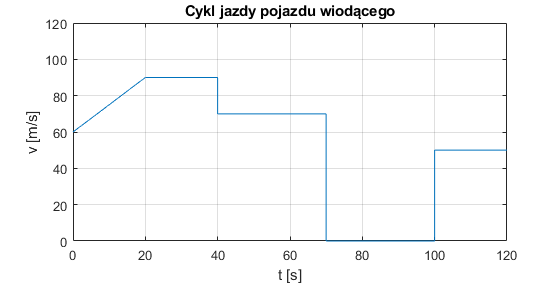
\includegraphics[width=.8\textwidth]{drvcycle.png}
	\caption{Cykl jazdy pojazdu wiodącego}
	\label{fig:drvc}
\end{figure}

Zadany cykl jazdy uwzględnia zmiany prędkości, pełne wyhamowanie i ponowne ruszenie.
Dodatkowo aby zasymulować wtargnięcie na jezdnię wykorzystano dodatkowy sygnał skokowy
o przebiegu (Rys. \ref{fig:dist_inter})

\begin{figure}[H]
	\centering
	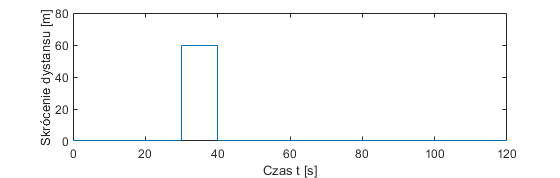
\includegraphics[width=.8\textwidth]{distinterupt.png}
	\caption{Przebieg funkcji skracającej dystans}
	\label{fig:dist_inter}
\end{figure}

Wtargnięcie jest realizowane poprzez odjęcie sygnału przedstawionego na Rys. \ref{fig:dist_inter}
od odległości pomiędzy pojazdami, przez co wymuszenie zahamowania na pojeździe podążającym.

\subsubsection{Wyniki symulacji}

\begin{figure}[H]
	\centering
	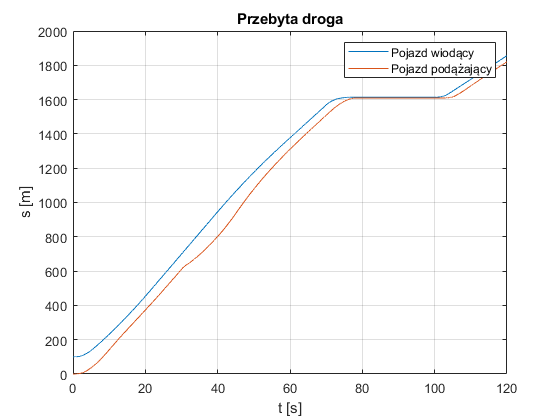
\includegraphics[width=.8\textwidth]{dstdrv.png}
	\caption{Przebieg przemieszczenia pojazdów}
	\label{fig:dist_driven}
\end{figure}

\begin{figure}[H]
	\centering
	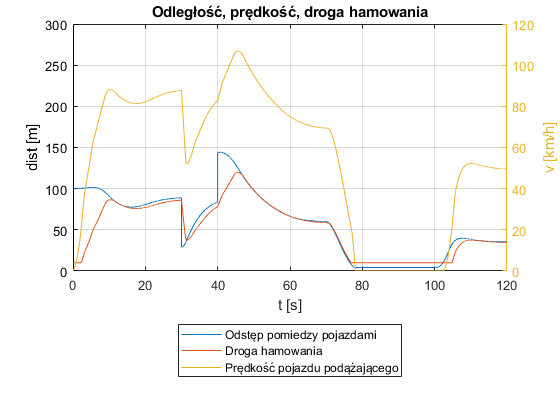
\includegraphics[width=.8\textwidth]{svbs.png}
	\caption{Przebiegi $\Delta s$, $v_{car1}$, $s_{hamowania}$}
	\label{fig:svbs}
\end{figure}

\begin{figure}[H]
	\centering
	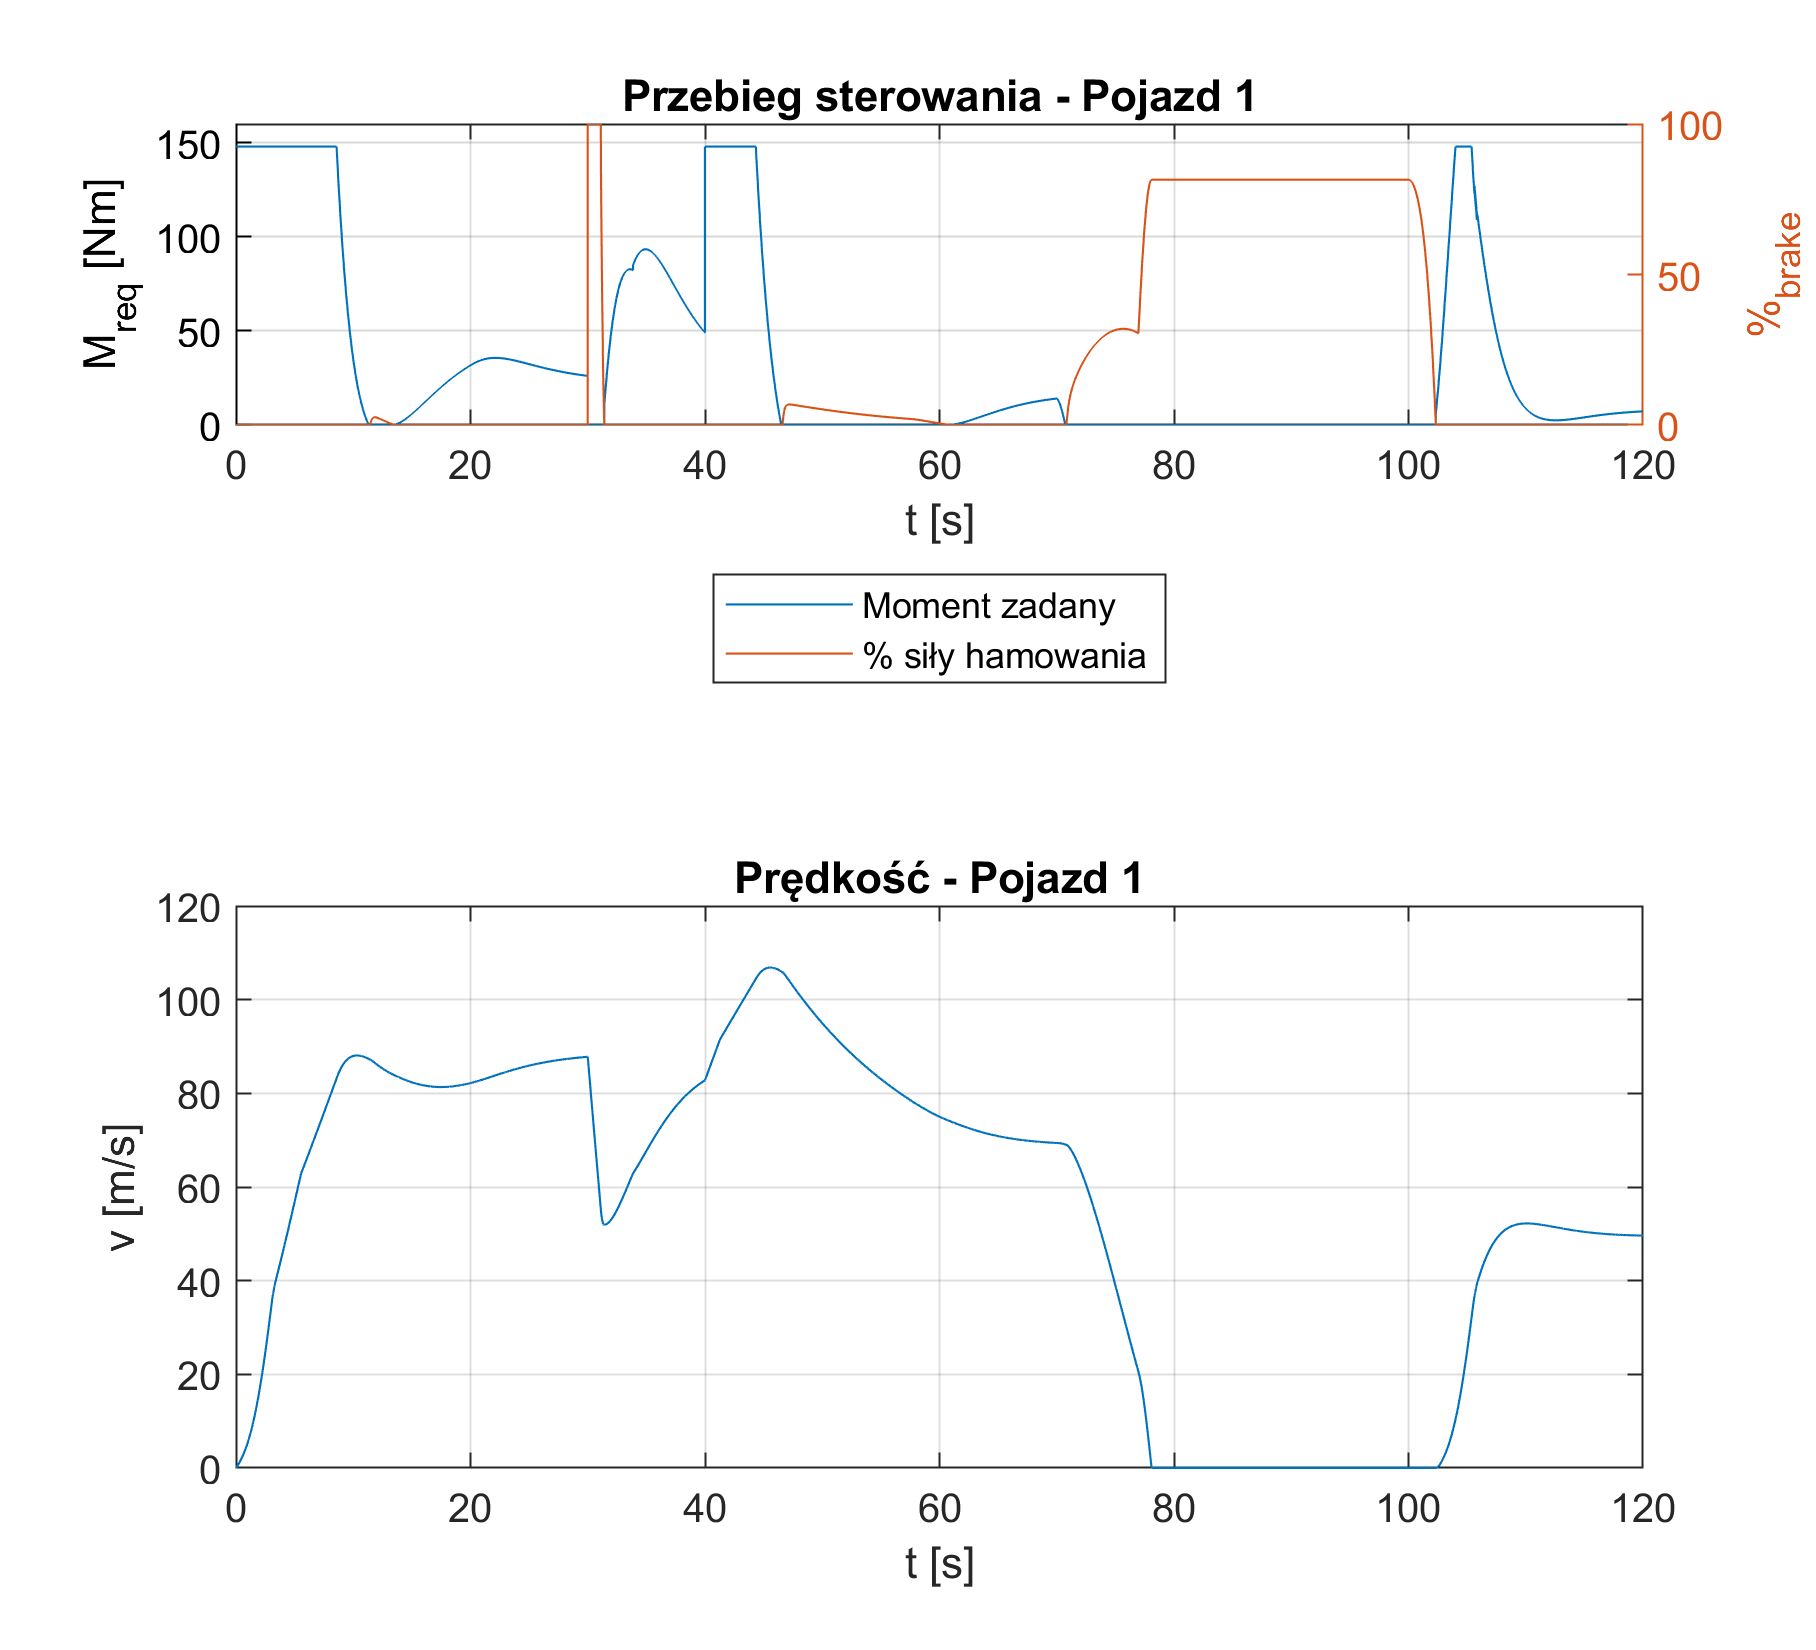
\includegraphics[width=.8\textwidth]{str_c1.png}
	\caption{Przebieg sterowania i prędkości pojazdu podążającego}
	\label{fig:strc1}
\end{figure}

\begin{figure}[H]
	\centering
	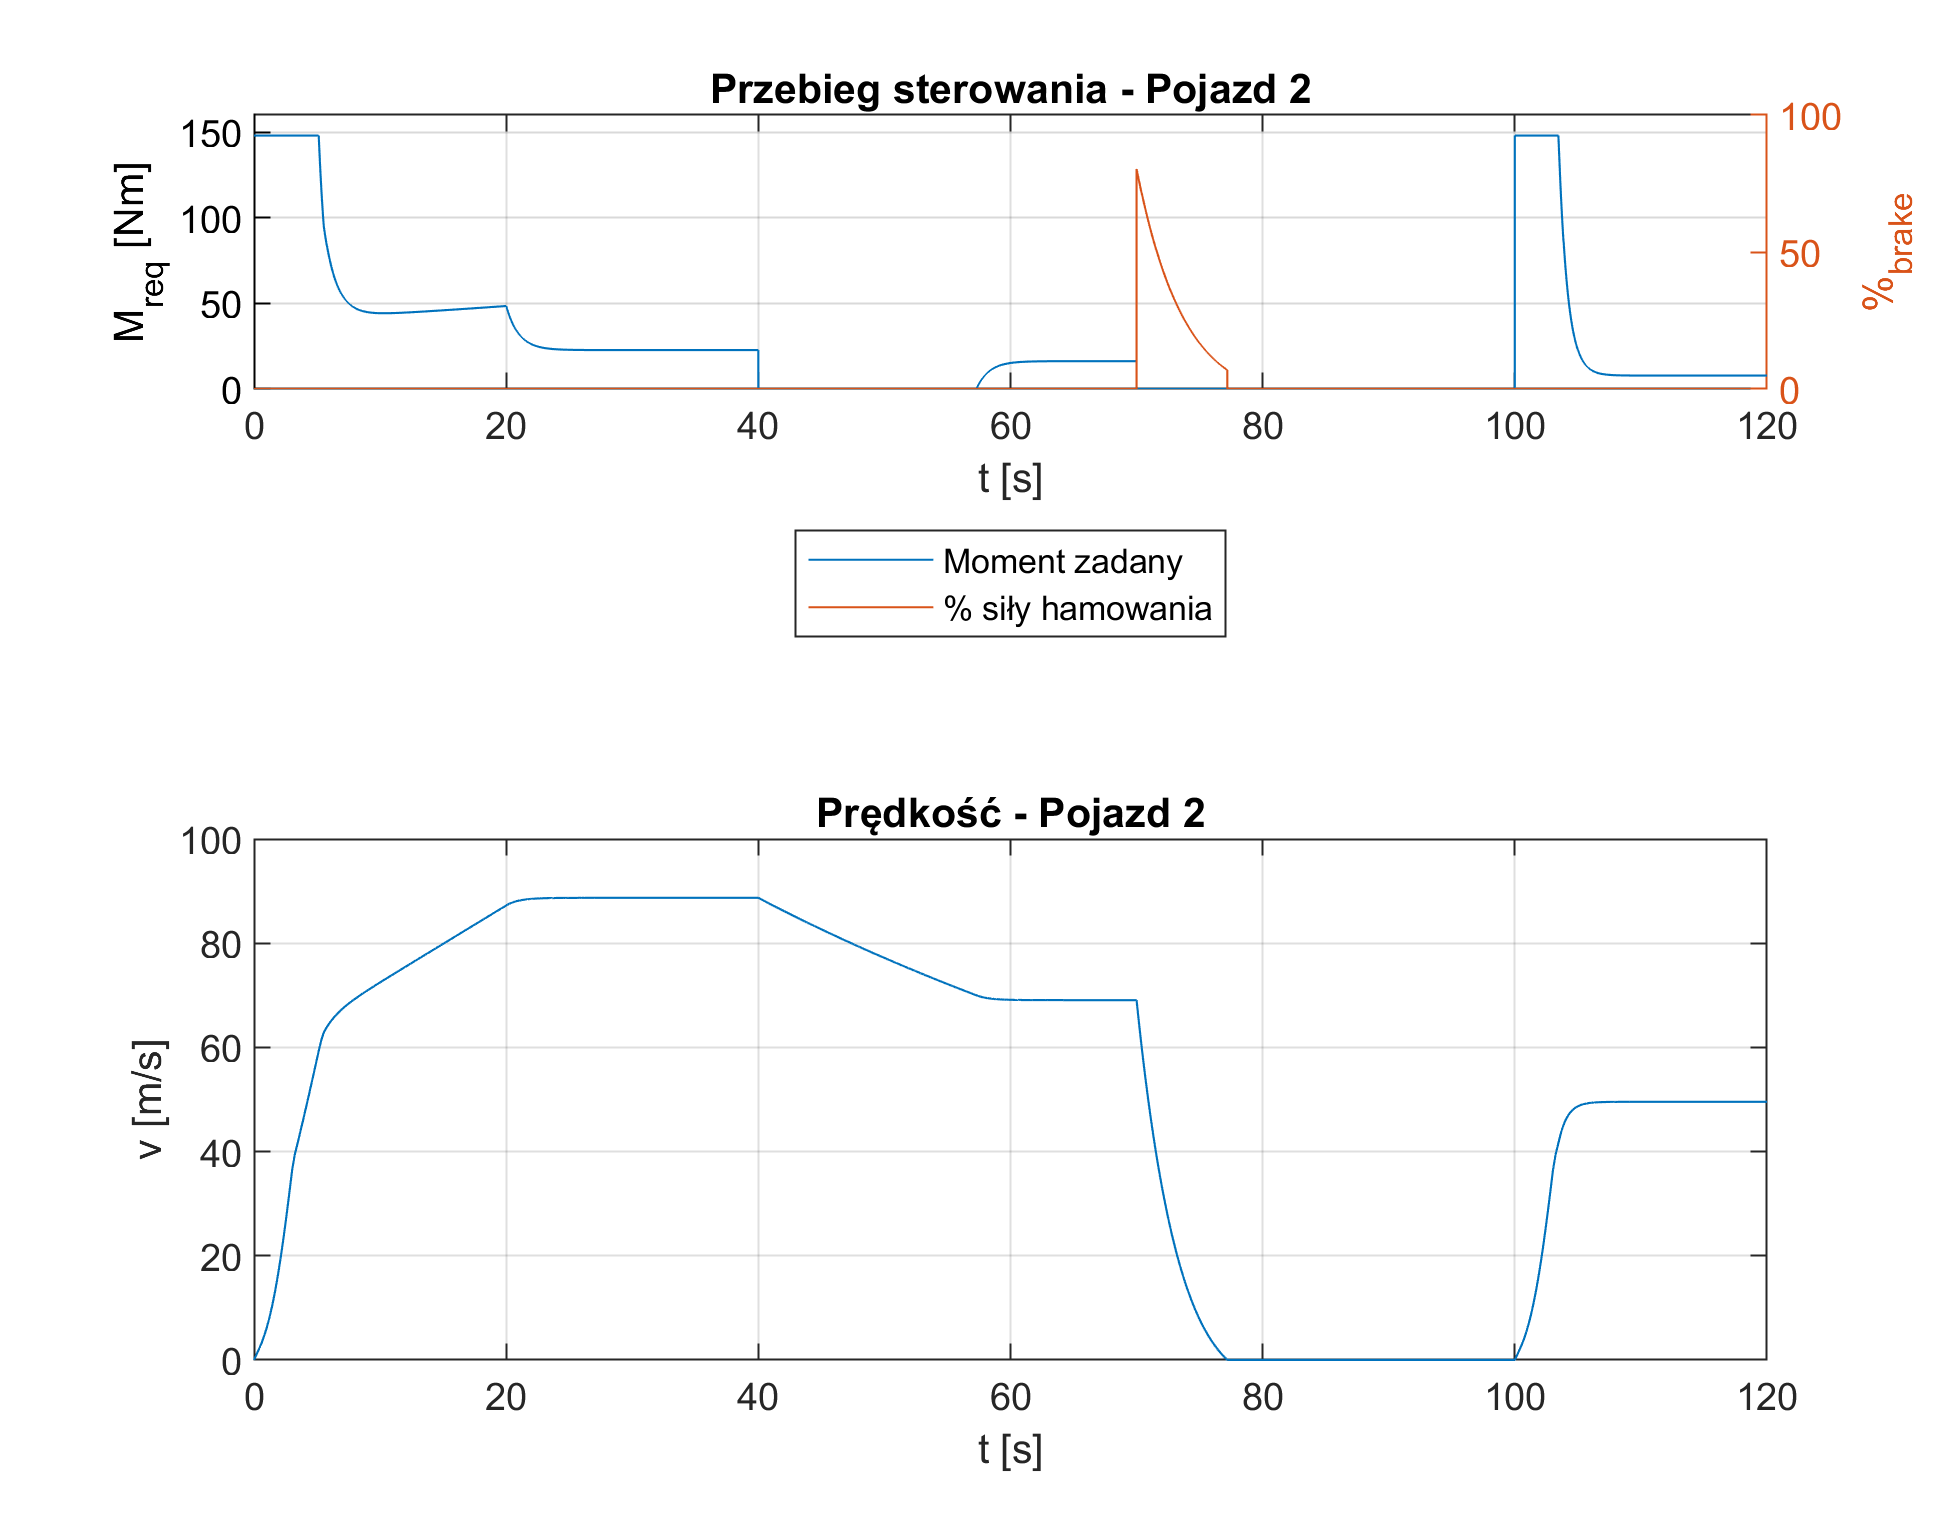
\includegraphics[width=.8\textwidth]{str_c2.png}
	\caption{Przebieg sterowania i prędkości pojazdu wiodącego}
	\label{fig:strc2}
\end{figure}


\begin{figure}[H]
	\centering
	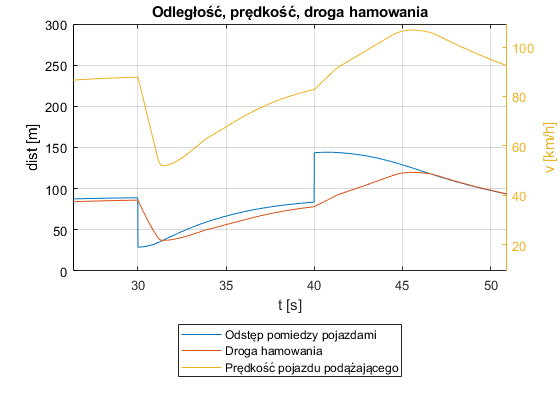
\includegraphics[width=.8\textwidth]{interupt.png}
	\caption{Zbliżenie na moment wtargnięcia na Rys. \ref{fig:svbs}}
	\label{fig:svbs_zoom}
\end{figure}

\subsubsection{Wnioski}

Układ realizuje sterowanie pojazdem podążającym w sposób płynny i zgodny z przyjętymi
założeniami, na Rys. \ref{fig:svbs_zoom} widać że w momencie wtargnięcia pojazd podążający
gwałtownie redukuje prędkość (na Rys. \ref{fig:strc1} sygnał sterujący układem hamulcowym 
gwałtownie skacze do 100\% intensywności siły hamowania). Pojazd
w trakcie poruszania się utrzymuje przez cały czas odpowiedni dystans określony
drogą hamowania dla danej prędkości poruszania się. Przyśpieszanie realizowane jest
w sposób płynny i z wartościami adekwatnymi do odległości między pojazdami.


\section{Podsumowanie}

Dzięki wykonaniu symulacji systemu mamy możliwość stworzenia funkcjonalnego prototypu
układu sterowania w sposób prosty nie wymagający zagłębiania się w specyfikę urządzeń,
na których docelowo układ ma być zrealizowany. Dzięki pełnej dowolności zadawania sygnałów
docierających do systemu możemy symulować sytuacje, których zrealizowanie innymi metodami
eksperymentalnymi byłoby bardzo kosztowne, niebezpieczne lub niemożliwe. Dzięki wbudowanym
możliwościom eksportu funkcjonalności stworzonych w środowisku \textit{MATLAB/Simulink}
do języka C możliwe jest wykorzystanie stworzonych fragmentów układu sterowania w 
kodzie źródłowym produkcyjnego rozwiązania układu.

\newpage
\section{Oświadczenie o samodzielności wykonania}

\textbf{Oświadczam} że niniejsza praca zaliczeniowa stanowiąca podstawę obecny
efektów uczenia się z przedmiotu \textit{Projektowanie Systemów Mechatronicznych} 
została przeze mnie wykonana samodzielnie.

\bigskip

\hfill Michał Łukaszewicz

\hfill \textit{297696}

\begin{thebibliography}{20} 
	\bibitem{arczy}
		S. Arczyński, \emph{Mechanika Ruchu Samochodu}\\
		Wydawnictwa Naukowo Techniczne, Warszawa 1994

	\bibitem{autocatalog}
		Mitsubishi Lancer 1.5 2009 - Strona internetowa
		\href{https://www.automobile-catalog.com/car/2009/1996115/mitsubishi_lancer_1_5.html}{Automobile Catalog}\\
		Data dostępu: 4.04.2021
\end{thebibliography}
   
\end{document}
